% This file was created with tikzplotlib v0.10.1.post5.
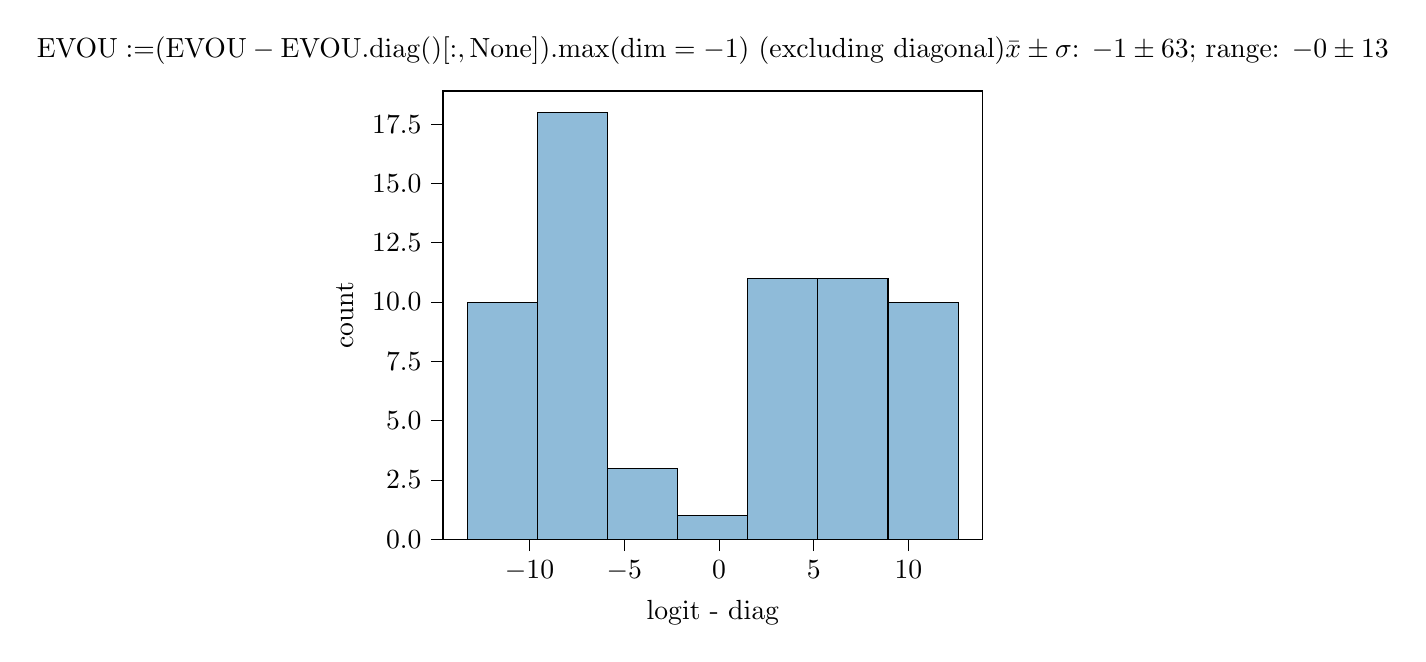
\begin{tikzpicture}

\definecolor{darkgray176}{RGB}{176,176,176}
\definecolor{steelblue31119180}{RGB}{31,119,180}

\begin{axis}[
tick align=outside,
tick pos=left,
title={\(\displaystyle \mathrm{EVOU} := \WE \WV \WO\WU \)\\
\(\displaystyle (\mathrm{EVOU} - \mathrm{EVOU}\mathrm{.diag}()[:,\mathrm{None}])\mathrm{.max}(\mathrm{dim}=-1)\) (excluding diagonal)\\
\(\displaystyle \bar{x}\pm\sigma\): \(\displaystyle -1 \pm 63\); range: \(\displaystyle -0 \pm 13\)},
x grid style={darkgray176},
xlabel={logit - diag},
xmin=-14.5656604766846, xmax=13.9137668609619,
xtick style={color=black},
xtick={-15,-10,-5,0,5,10,15},
xticklabels={
  \(\displaystyle {\ensuremath{-}15}\),
  \(\displaystyle {\ensuremath{-}10}\),
  \(\displaystyle {\ensuremath{-}5}\),
  \(\displaystyle {0}\),
  \(\displaystyle {5}\),
  \(\displaystyle {10}\),
  \(\displaystyle {15}\)
},
y grid style={darkgray176},
ylabel={count},
ymin=0, ymax=18.9,
ytick style={color=black},
ytick={0,2.5,5,7.5,10,12.5,15,17.5,20},
yticklabels={
  \(\displaystyle {0.0}\),
  \(\displaystyle {2.5}\),
  \(\displaystyle {5.0}\),
  \(\displaystyle {7.5}\),
  \(\displaystyle {10.0}\),
  \(\displaystyle {12.5}\),
  \(\displaystyle {15.0}\),
  \(\displaystyle {17.5}\),
  \(\displaystyle {20.0}\)
}
]
\draw[draw=black,fill=steelblue31119180,fill opacity=0.5] (axis cs:-13.2711410522461,0) rectangle (axis cs:-9.57251412527902,10);
\draw[draw=black,fill=steelblue31119180,fill opacity=0.5] (axis cs:-9.57251412527902,0) rectangle (axis cs:-5.87388719831194,18);
\draw[draw=black,fill=steelblue31119180,fill opacity=0.5] (axis cs:-5.87388719831194,0) rectangle (axis cs:-2.17526027134487,3);
\draw[draw=black,fill=steelblue31119180,fill opacity=0.5] (axis cs:-2.17526027134487,0) rectangle (axis cs:1.52336665562221,1);
\draw[draw=black,fill=steelblue31119180,fill opacity=0.5] (axis cs:1.52336665562221,0) rectangle (axis cs:5.22199358258928,11);
\draw[draw=black,fill=steelblue31119180,fill opacity=0.5] (axis cs:5.22199358258928,0) rectangle (axis cs:8.92062050955636,11);
\draw[draw=black,fill=steelblue31119180,fill opacity=0.5] (axis cs:8.92062050955636,0) rectangle (axis cs:12.6192474365234,10);
\end{axis}

\end{tikzpicture}
